\chapter{Μοντέλο πρόβλεψης απόδοσης απαντήσεων βάσει προτροπής}
\label{ch:chapter4}

Στο Κεφάλαιο \ref{ch:chapter3} παρουσιάστηκε η μεθοδολογία που
ακολουθήθηκε για την συλλογή των δεδομένων και την αξιολόγηση των
απαντήσεων του μοντέλου του \textlatin{GitHub Copilot}. Η
κατηγοριοποίηση των δεδομένων, οδήγησε στην ιδέα να αναπτυχθεί ένα
μοντέλο μηχανικής μάθησης με σκοπό την πρόβλεψη της απόδοσης μιας
απάντησης του μοντέλου του \textlatin{GitHub Copilot}, με βάση την
προτροπή.

Με βάση την προτροπή, αρχικά έγινε η προσπάθεια για την πρόβλεψη της
ακριβούς τιμής της αξιολόγησης, από πολύ αρνητική έως πολύ θετική, αλλά,
λόγω του μικρού μεγέθους των δεδομένων, η παραπάνω λογική οδήγησε σε
εξαιρετικά ασυνεπή αποτέλεσματα, με ακρίβεια χαμηλότερη αυτής των
πενήντα τοις εκατό (50\%). Συνεπώς, αποφασίστηκε να γίνει η προσπάθεια
κατηγοριοποίησης της απάντησης είτε σε θετική αξιολόγηση, είτε σε
αρνητική.

\section{Κατηγοριοποίηση των δεδομένων}

Για την κατηγοριοποίηση των δεδομένων, η κάθε προτροπή επεξεργάστηκε,
προκειμένου να αφαιρεθούν τα κομμάτια κώδικα από την υπόλοιπη προτροπή
και έπειτα αφαιρέθηκαν οι "κενές λέξεις" (\textlatin{stopwords}) με την
χρήση της βιβλιοθήκης \textlatin{Natural Language Toolkit (NLTK)}. Για
κάθε προτροπή που είχε κομμάτια κώδικα, ο αριθμός των συμβόλων
(\textlatin{symbols}), αποθηκεύθηκε σε μια άλλη κατηγορία.

Ένα από τα μεγαλύτερα προβλήματα των Γλωσσικών Μοντέλων, είναι ο
μέγιστος αριθμός των συμβόλων (\textlatin{tokens}) που μπορούν να
επεξεργαστούν. Καθώς οι προτροπές ζητούσαν μεγάλα κώδικα, ειδικά στις
περιπτώσεις των ελέγχων του κώδικα, το μοντέλο συχνά έφτανε στο όριο των
δεδομένων που μπορούσε να παράξει στην απάντησή του. Καθώς το μοντέλο
δεν γνώριζε εκ των προτέρων το μέγεθος της απάντησης, αν ο
προγραμματιστής δεν το παρότρυνε να σταματήσει σε ένα συγκεκριμένο
αριθμό συμβόλων, το μοντέλο θα συνέχιζε να παράγει κώδικα μέχρι να
φτάσει στο όριο των δεδομένων που μπορούσε να παράξει, οδηγώντας σε μια
σειρά από αποτυγχημένες απαντήσεις.

Για την αντιμετώπιση του προβλήματος, ο προγραμματιστής ζήτησε από το
μοντέλο να απαντάει για ένα συγκεκριμένο μέρος του προβλήματος, όπως
παραδείγματος χάρη έναν συγκεκριμένο έλεγχο, αντί όλων των ελέγχων.
΄Επειτα, ζήτησε από το το μοντέλο να περιμένει την προτροπή με
περιεχόμενο την λέξη "\textlatin{continue}" (συνέχισε), προκειμένου να
συνεχίσει με την προηγούμενη απάντησή του. Με αυτόν τον τρόπο, το
μοντέλο θα μπορούσε να απαντήσει σε μια προτροπή, χωρίς να φτάσει στο
όριο των δεδομένων που μπορούσε να παράξει.

Ωστόσο, αυτό οδήγησε σε αρκετές προτροπές με μοναδικό περιεχόμενο την
λέξη "\textlatin{continue}", που αφενός δεν είχαν καμία σχέση με το
προηγούμενο κείμενο και αφετέρου, εφ᾽ όσον ο προγραμματιστής παρότρυνε
το μοντέλο να συνεχίσει με την απάντησή του, σήμαινε πως η τουλάχιστον
αμέσως προηγούμενη απάντηση ήταν ικανοποιητική, οδηγώντας σε μια
μεροληψία προς θετικά αποτελέσματα. Συνεπώς, αποφασίστηκε να
υπολογίζεται ο συνεχόμενος αριθμός προτροπών με περιεχόμενο την λέξη
"\textlatin{continue}", συνάμα με το θέμα της προτροπής, ώστε να
δημιουργούνται ομάδες προτροπών που στοχεύουν στο ίδιο ερώτημα, αλλά
χρειάστηκε να διασπαστούν λόγω των περιορισμών του μοντέλου.

Περιπτώσεις προτροπών που είτε ματαιώθηκαν, είτε δεν είχαν απάντηση λόγω
τεχνικών προβλημάτων, ήταν σημειωμένες εξαρχής και παραλείφθηκαν από την
ανάλυση.

\subsection{Προεπεξεργασία και Προετοιμασία Δεδομένων}

Με την χρήση των βιβλιοθηκών \texlatin{pandas} και
\texlatin{scikit-learn}, η διαδικασία προεπεξεργασίας και προετοιμασίας
των δεδομένων περιελάμβανε τα ακόλουθα στάδια:
\begin{enumerate}
\item
  \textbf{Εισαγωγή Δεδομένων:} Τα δεδομένα εισήχθησαν από ένα αρχείο CSV
  χρησιμοποιώντας τη βιβλιοθήκη \texlatin{pandas} για τον αποτελεσματικό
  χειρισμό τους.
\item
  \textbf{Κωδικοποίηση Κατηγορικών Μεταβλητών:} Οι κατηγορικές
  μεταβλητές "\textlatin{subject}" (θέμα) και "\textlatin{type}" (τύπος)
  κωδικοποιήθηκαν αριθμητικά με τη χρήση του \textlatin{LabelEncoder}.

\item
  \textbf{Μετατροπή Χρονικών Δεδομένων:} Η στήλη \textlatin{"createdAt"}
  μετατράπηκε σε αριθμητική μορφή, αντιπροσωπεύοντας τα δευτερόλεπτα από
  την εποχή \textlatin{UNIX} (1/1/1970).

\item
  \textbf{Δυαδικοποίηση Αξιολογήσεων:} Η στήλη \textlatin{"rating"}
  (αξιολόγηση) μετατράπηκε σε δυαδική μορφή, όπου οι θετικές
  αξιολογήσεις αντιστοιχήθηκαν στην τιμή ένα (1) και οι αρνητικές στην
  τιμή μηδέν (0).

\item
  \textbf{Ομαδοποίηση Δεδομένων:} Πραγματοποιήθηκε ομαδοποίηση των
  δεδομένων με βάση τη στήλη \textlatin{"group"}. Για κάθε ομάδα,
  υπολογίστηκαν διάφορα στατιστικά μέτρα, όπως ο μέσος όρος για τις
  αριθμητικές μεταβλητές και η επικρατούσα τιμή για τις κατηγορικές.

\item
  \textbf{Επεξεργασία Κειμένου:} Εφαρμόστηκε η τεχνική \textlatin{Term
    Frequency-Inverse Document Frequency (TF-IDF)} για τη μετατροπή των
  κειμενικών προτροπών σε αριθμητικά χαρακτηριστικά. Η στήλη
  \textlatin{"prompt"} (προτροπή) μετασχηματίστηκε σε πολλαπλές στήλες,
  κάθε μία εκ των οποίων αντιπροσωπεύει ένα διακριτό χαρακτηριστικό
  \textlatin{TF-IDF}.

\item
  \textbf{Διαχείριση Ελλιπών Τιμών:} Οι ελλιπείς τιμές στις αριθμητικές
  στήλες αντικαταστάθηκαν με τη μέση τιμή της αντίστοιχης στήλης,
  διασφαλίζοντας την πληρότητα του συνόλου δεδομένων.
\end{enumerate}

\subsection{Επιλογή Χαρακτηριστικών}

Η διαδικασία επιλογής χαρακτηριστικών περιελάμβανε τα εξής βήματα:
\begin{enumerate}
\item
  \textbf{Εφαρμογή \textlatin{SelectKBest}:} Χρησιμοποιήθηκε η μέθοδος
  \textlatin{SelectKBest} σε συνδυασμό με τη συνάρτηση (${\chi}^2$) για
  την επιλογή των δέκα (10) πιο σημαντικών χαρακτηριστικών. Αυτή η
  προσέγγιση συνέβαλε στη μείωση της διαστατικότητας του προβλήματος και
  στην επικέντρωση στα πλέον πληροφοριακά χαρακτηριστικά.

\item
  \textbf{Διαχωρισμός Δεδομένων:} Τα δεδομένα διαχωρίστηκαν σε σύνολα
  εκπαίδευσης και ελέγχου, με αναλογία ογδόντα τοις εκατό (80\%) και
  είκοσι τοις εκατό (20\%) αντίστοιχα, χρησιμοποιώντας τη συνάρτηση
  \textlatin{train\_test\_split}.
\end{enumerate}

\section{Εκπαίδευση και Αξιολόγηση Μοντέλων}

Για την εκπαίδευση και αξιολόγηση των μοντέλων ακολουθήθηκε η εξής
διαδικασία:
\begin{enumerate}
\item
  \textbf{Επιλογή Αλγορίθμων:} Επιλέχθηκαν τέσσερις διαφορετικοί
  αλγόριθμοι μηχανικής μάθησης: \tl{Random Forest, Support Vector
    Machine (SVM), Gradient Boosting}, και \tl{Naive Bayes}.
\item
  \textbf{Βελτιστοποίηση Υπερπαραμέτρων:} Για κάθε αλγόριθμο,
  πραγματοποιήθηκε εκτενής αναζήτηση πλέγματος (\tl{Grid Search}) με
  δεκάπτυχη διασταυρωμένη επικύρωση για τη βελτιστοποίηση των
  υπερπαραμέτρων.

\item
  \textbf{Εκπαίδευση Μοντέλων:} Τα μοντέλα εκπαιδεύτηκαν χρησιμοποιώντας
  τις βέλτιστες υπερπαραμέτρους που προέκυψαν από την αναζήτηση
  πλέγματος.

\item
  \textbf{Αξιολόγηση Μοντέλων:} Η απόδοση των μοντέλων αξιολογήθηκε
  χρησιμοποιώντας το σύνολο ελέγχου. Υπολογίστηκαν μετρικές όπως η
  ακρίβεια, η ανάκληση, και το \tl{F1-score}.

\item
  \textbf{Οπτικοποίηση Αποτελεσμάτων:} Δημιουργήθηκαν πίνακες σύγχυσης
  (\tl{confusion matrices}) και συγκριτικά γραφήματα για την οπτική
  αναπαράσταση της απόδοσης των διαφόρων μοντέλων.
\end{enumerate}
Η μεθοδολογία αυτή επέτρεψε τη συστηματική ανάπτυξη, εκπαίδευση και
αξιολόγηση των μοντέλων, παρέχοντας μια ολοκληρωμένη εικόνα της απόδοσής
τους στην ταξινόμηση των δεδομένων.

Πραγματοποιήθηκε επίσης έρευνα για την επιλογή ανάπτυξης ενός νευρωνικού
δικτύου, αλλά λόγω του μικρού μεγέθους των δεδομένων, το αποτέλεσμα ήταν
ανεπαρκή, με ακρίβεια κάτω του πενήντα τοις εκατό (50\%). Με την
εφαρμογή των παραπάνω βημάτων, η ακρίβεια των μοντέλων αυξήθηκε
σημαντικά, με τα αποτελέσματα να αναλύονται παρακάτω.

\section{Αποτελέσματα}

Η ανάπτυξη ενός μοντέλου πρόβλεψης της απόδοσης Γλωσσικών Μοντέλων βάσει
πολλαπλών κριτηρίων, με ιδιαίτερη έμφαση στην προτροπή, αποτελεί ένα
καινοτόμο ερευνητικό εγχείρημα. Ο όρος "μηχανική προτροπής"
(\textlatin{Prompt Engineering}) αναφέρεται στη εξειδικευμένη
μεθοδολογία σχεδιασμού και βελτιστοποίησης προτροπών με στόχο τη
μεγιστοποίηση της απόδοσης του μοντέλου \cite{10.1162/tacl_a_00324,
  chen2024unleashingpotentialpromptengineering}.

Οι επιστημονικές έρευνες στον ραγδαία εξελισσόμενο τομέα αυτό είναι
ιδιαίτερα πρόσφατες, με την πλειονότητα των σημαντικών δημοσιεύσεων να
εμφανίζεται μετά τη δημόσια κυκλοφορία του \textlatin{ChatGPT}
\cite{greshake2023youvesignedforcompromising,
  white2023promptpatterncatalogenhance}. Ωστόσο, η αποτελεσματική
εφαρμογή και βελτιστοποίηση της μηχανικής προτροπής αποτελεί ένα από τα
πιο κρίσιμα και πολύπλοκα προβλήματα ενός κόσμου ολοένα και περισσότερο
ενισχυμένου από την τεχνητή νοημοσύνη.

Η εξαγωγή του μέγιστου δυνατού επιπέδου απόδοσης από τα Γλωσσικά
Μοντέλα, και κατ' επέκταση η μείωση σφαλμάτων και μη ικανοποιητικών
αποκρίσεων, με αποτέλεσμα την αποτελεσματική αύξηση της απόδοσης χωρίς
την εισαγωγή επιπρόσθετων δεδομένων ή την τροποποίηση του υπάρχοντος
κώδικα ανάπτυξης του μοντέλου, αποτελεί μια διαδικασία τόσο δύσκολη όσο
και δυσνόητη. Η αξιοποίηση ενός μοντέλου μηχανικής μάθησης για την
πρόβλεψη της απόδοσης ενός γλωσσικού μοντέλου βάσει της προτροπής
δύναται να παράσχει πολύτιμα εργαλεία για τη μεγιστοποίηση της απόδοσης.

\begin{figure}[H]
  \begin{center}
    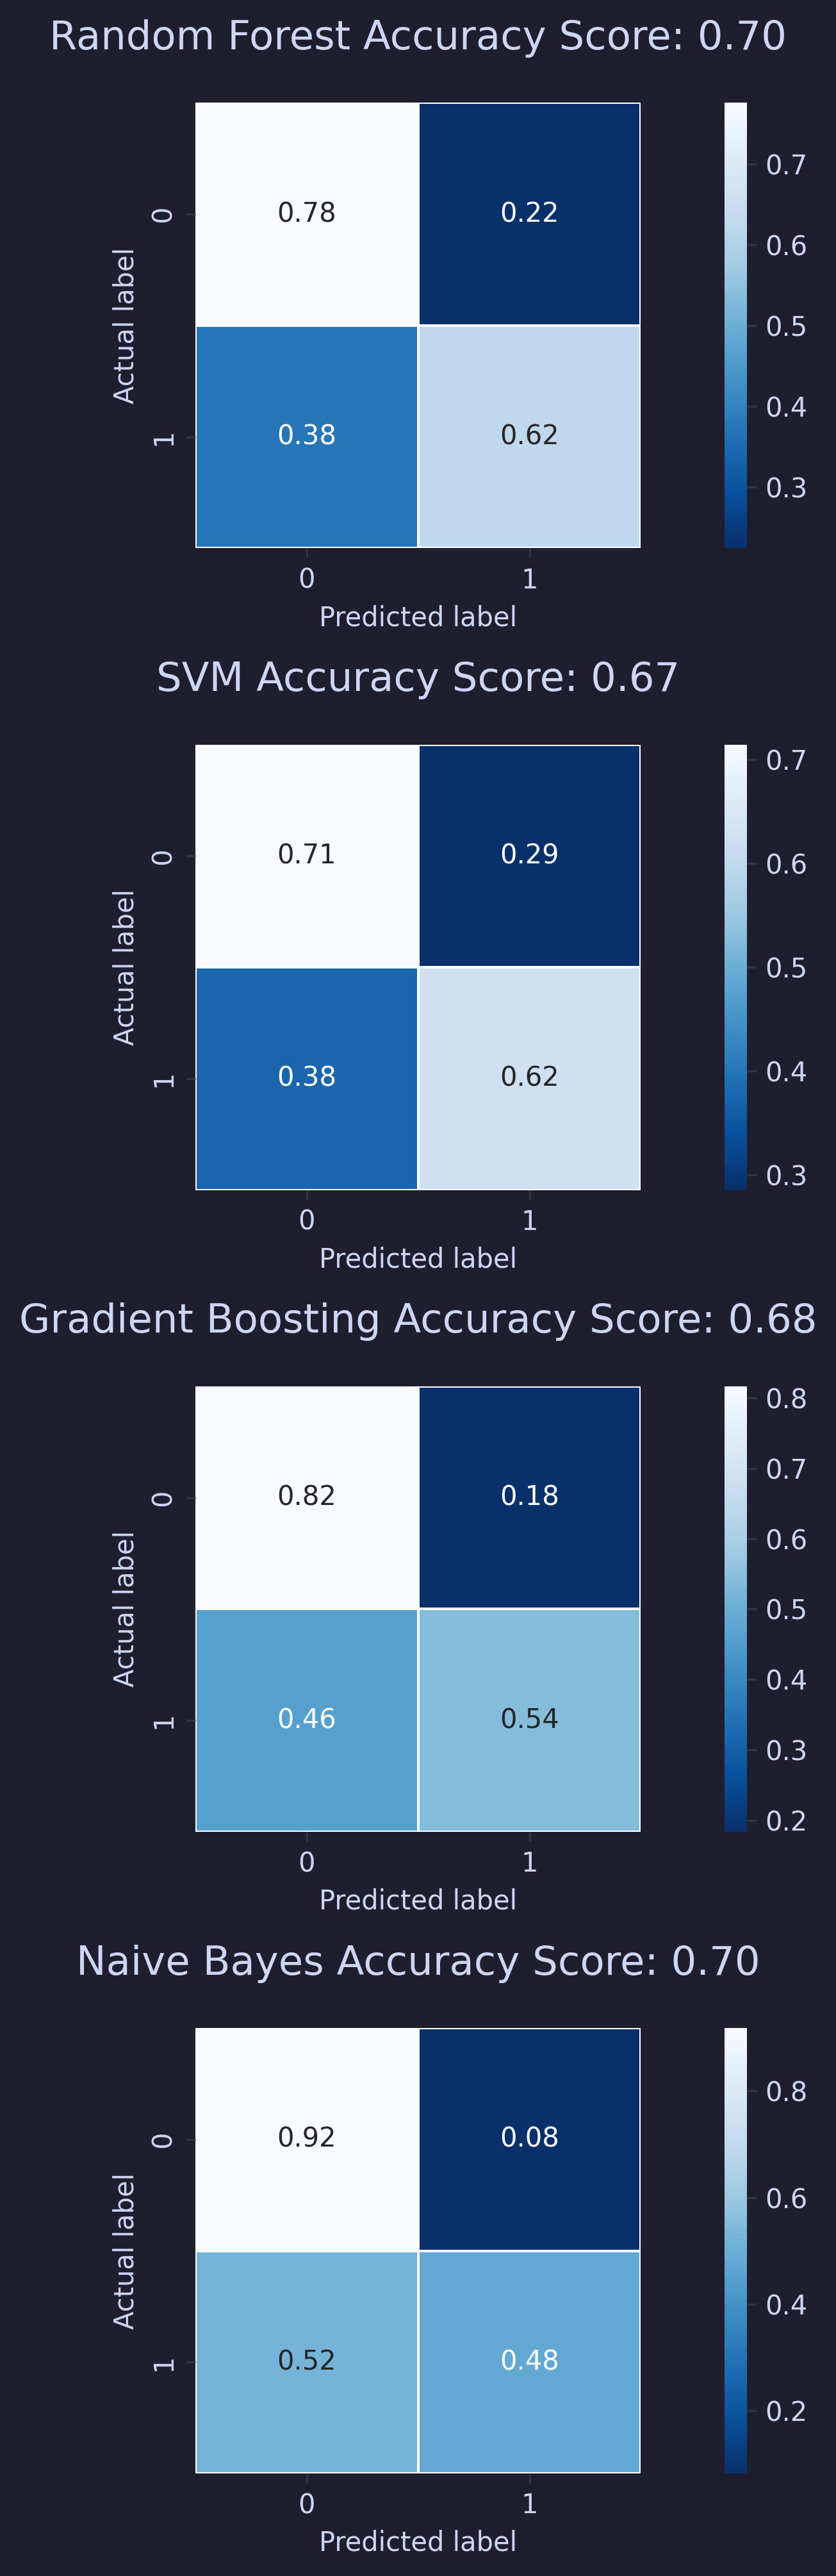
\includegraphics[width=0.85\textwidth]{confusion_matrix.png}
    \caption{Μέσος όρος αξιολόγησης απαντήσεων για θέματα, \textit{μέρος
        3}}
  \end{center}
  \label{fig:SubjectQuery3}
\end{figure}
